\chapter{aparimeVya saMKeyxgaLu}
%\vskip -20pt

$ 4,9,16,25\cdots$ muMtAda saMKeyxgaLu pUNaRvagaR saMKeyxgaLu. ivugaLige pUNaR\-vagaR mUlagaLive. Adare $2,3,5,7$ muMtAda saMKeyxgaLige pUNaRvagaRmUlaviruvudilalx ivelAlx ivelAlx apameVriya saMKeyxgaLu. I riVtiya saMKeyxgaLige vagaRmUla\-vanunx kaMDu hiDiyalu sAdhayxvilalx. AdarU sariyAda utatxrakekx samiVpada bele\-yanunx kaMDuhiDiyabahudu.

\textbf{udAharaNege:} \qquad $2$ ra vagaRmUla
$$
\sqrt{2} = 1.41421
$$
$2$ ra vagaRmUlavanunx $5$ dashamAMsha sAthxnadavarege bareyalAgide. idanunx hiVgeyeV muMduvarisabahudu I riVtiya saMKeyxgaLanunx aparimeVya saMKeyxgaLu enunxtetxVve.

\medskip
peYthAgorasfna parxmeVyada parxkAra {\bf aparimeVya saMKeyxgaLa vagaRmUlavanunx} reVKAgaNitada riVti kaMDuhiDiyabahudu.

peYthAgorasana parxmeVya namagelAlx tiLidide. 

laMbakoVna tirxBujadalilx vikaNaRda meVlina vagaRvu uLideraDu bAhugaLa vagaRgaLa motatxkekx sama.

\begin{tabular}[c]{>{$}l<{$}}
\includegraphics{src/figure/m_049.eps}
\end{tabular}
\hspace{0.2cm}
\begin{tabular}[c]{>{$}l<{$}}
OAB\quad \text{oMdulaMbakoVna tirxBuja}\\
O\widehat{A}B = 90^{\circ}\\
OA \;\text{matutx}\; AB \;\text{oMdu seMmiV Adare}\\ 
\text{peYthAgorasfna parxmeVyada parxkAra}
\end{tabular}

\begin{align*}
OB^2 &= OA^2+AB^2\\
&= 1^2+1^2\\
&= 1+1\\
OB^2 &= 2\\
\therefore OB &= \sqrt{2}
\end{align*}
vikaNaR $OB$ ya udadxvanunx ALedAga $\sqrt{2}$ ra belegotAtxgutatxde.

\begin{tabular}[c]{>{$}l<{$}}
\includegraphics{src/figure/m_051.eps}
\end{tabular}
\begin{tabular}[c]{>{$}l<{$}}
\text{Iga}\; OBC \;\text{tirxBujadalilx}\;  \widehat{B} = 90^{\circ}\\
OB=\sqrt{2}, BC = 1 \;\text{seMmiV}
\end{tabular}
\begin{align*}
OC^2 &= OB^2+BC^2\\
&= (\sqrt{2})^2+(\sqrt{1})^2\\
&=2+1\\
OC^2&= 3\\
\therefore OC &= \sqrt{3}
\end{align*}

$3$ oMdu aparimeVya saMKeyx adara vagaRmUlavanunx $OC$ yanunx aLeyuva mUlaka tiLiyabahudu.

\begin{tabular}[l]{>{$}l<{$}}
\includegraphics{src/figure/m_051a.eps}
\end{tabular}
\begin{tabular}[c]{>{$}l<{$}}
\text{Iga}\;OCB\; \text{tirxBujadalilx}\;\widehat{c} = 90{\circ}\\
OC=\sqrt{3}, CD = 1 \;\text{seMmiV}
\end{tabular}
\begin{align*}
OD^2 &= OC^2+CD^2\\
&= (\sqrt{3})^2+(\sqrt{1})^2\\
&=3+1\\
OD^2&= 4\\
\therefore\ OD &= \sqrt{4}\\
&= 2
\end{align*}
hiVgeyeV muMduvarisidare $5,6,7,8,9,10$ ra {\bf vagaR mUlavanunx kaMDuhiDiya\-bahudu.}

meVle heVLiruva saMKeyxgaLalilx $5,6,7,8,10$ ivugaLelAlx aparimeVya saMKeyxgaLu.
\begin{flalign*} 
\quad\qquad\sqrt{1}&=1.000&\\
\sqrt{2}&=1.414\\
\sqrt{3}&=1.732\\
\sqrt{4}&=2.000\\
\end{flalign*}

peY idoMdu aBAgalabadhxsaMKeyx. idu uyAvudeV vaqtatxda paridhigU matutx vAyxsakxkUkx iruva parxmANa (niSaTxtitx) idarabele $\frac{22}{7}$ athavA $3.146$ ra samiVpa. idara beleyanunx tiLiyalu vishavxdAdayxMta bahaLa hiMdina dinagaLiMda parxyatanxgaLu baDedive. kirx.~sha.\ $5$ neV shatamAnadalilxdadx BAratada suparxsidadhx gaNitajacnx AyaRBaTana parxkAra idara bele sUmAru $3.1416\ldots$. BAratada eraDaneya BAsakxrAcAyaRrU idara beleyanunx gaNitajacnx shirxVnivAsa rAmAnujanf saha samiVkaraNada rUpadalilx idara bele tiLisidAdxne. jAyxmitiya AkaqtigaLanunx baLasi idara beleyanunx nidhaRrisalu AraMBisidAdxre. 

vijAcnxna, taMtarxjAcnxna, gaNita matutx itara keSxVtarxgaLalilx $\pi$ nunx gaNitiVya sithxra saMKeyx\-yAgi nAvu baLasutitxdedxVve. 

ameVrikAdalilx mAcfR $14$ raMdu peYdinavAgi AcarisutAtxre. $(3.14)$ yUroVpf nalilx juleY $22$ raMdu peYdinavAgi AcarisutAtxre. $(\frac{22}{7})$ beVre beVre deVshagaLalilx vividha dinagaLaMdu AcarisutAtxre.

$e$ idoMdu aBAgalabadhx saMKeyx {\rm exponential} eMba iMgilxVSf padada modala\-neya akaSxra. idara bele $2.7182\cdot$

gaNitadalilx baruva lAgaridaMge ideV AdhAra. idanunx lAgaridaMnalilx baLasidavanu jAnf neVpiyarf.

ititxVcege BwtashAsatxrX, rasAyanashAsatxrX, jiVvashAsatxrX matutx samAna vijAcnxna muMtAda keSxVtarxgaLalilx $e$ nunx baLasutAtxre.

